\section{Implementation}
\label{sec:implementation}

\parabf{Overview.}
\spork{} is implemented in Python as a controller layer plus an optional D3 proposer
integration.
The D1/D2 path (fork dispatch, logprob monitoring, asynchronous tool execution, and
gate verification) uses standard OpenAI-compatible vLLM endpoints
(\texttt{/v1/chat/completions} for the main stream, \texttt{/v1/completions} for the fork).
D3 adds a small \texttt{SporkProposer} integration with vLLM's speculative-decoding
proposer path so that verified probe tokens can be injected as draft tokens at the
tool-call boundary.
Algorithm~\ref{alg:spork} summarizes the end-to-end control flow.
The HTTP controller realizes D1+D2; the engine configuration additionally performs D3,
which the HTTP path omits.

\begin{algorithm}[t]
\caption{\spork{} Controller with D1+D2+D3}
\label{alg:spork}
\begin{algorithmic}[1]
\REQUIRE User request, tool set $\mathcal{T}$, threshold $\theta$, retry budget $R$, token step $s$
\STATE Dispatch main stream (streaming chat completions)
\STATE Wait for main's first streaming token
\STATE $\mathrm{spec} \gets \emptyset$;\ $(\hat{t},\hat{a}) \gets \emptyset$
\FOR{$r = 0,1,\dots,R-1$}
\STATE Wait until main has decoded $r\cdot s$ further CoT tokens
\STATE Fork a completions request with forced prefix over observed CoT \COMMENT{D1 cache hit}
\STATE $(\hat{t},\hat{a}) \gets \mathrm{parse}(\mathrm{fork})$;\ $c \gets \min_{j \in \mathrm{name\_span}} \exp(\ell_j)$ \COMMENT{D2}
\IF{$(\hat{t},\hat{a})$ valid \AND $c \geq \theta$}
\STATE $\mathrm{spec} \gets \mathrm{async\_tool}(\hat{t},\hat{a})$ \COMMENT{commit; overlaps main decode}
\STATE \textbf{break}
\ENDIF
\IF{main stream finished}
\STATE \textbf{break}
\ENDIF
\ENDFOR
\STATE Wait for main tool call $(t^*,a^*)$
\IF{$\mathrm{spec}\neq\emptyset$ \AND $(\hat{t},\hat{a}) = (t^*,a^*)$}
\STATE \textbf{return} pre-computed $\mathrm{spec}$ result \COMMENT{strict match}
\ELSE
\STATE \textbf{return} $\mathrm{tool}(t^*,a^*)$ \COMMENT{serial fallback; D3 draft-injects the probe body during decode}
\ENDIF
\end{algorithmic}
\end{algorithm}

\begin{figure*}[t]
  \centering
  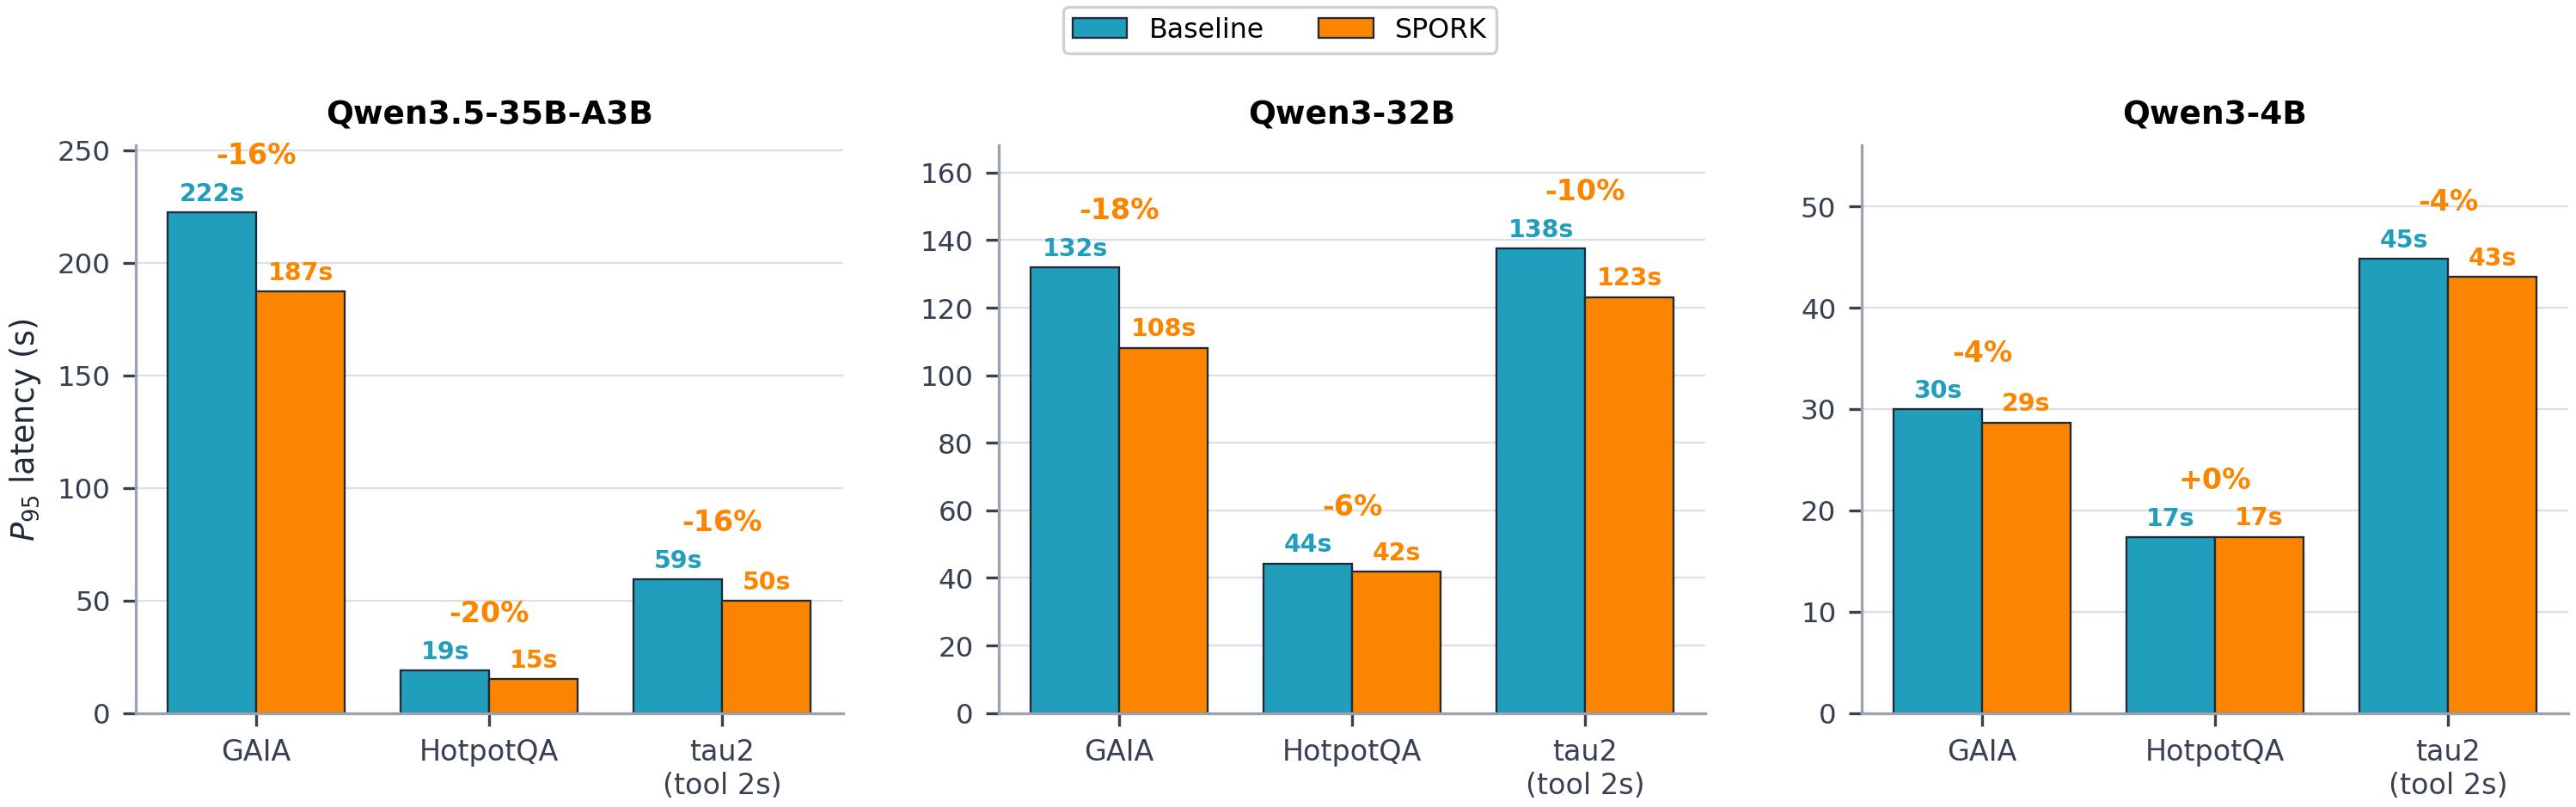
\includegraphics[width=0.84\textwidth]{figures/fig_hero_e2e_speedup.png}
  \caption{\textbf{\spork{} reduces $P_{95}$ tail latency across models and benchmarks.}
  Teal: baseline; orange: the paper-facing \spork{} configuration for each run
  (engine D1+D2+D3; HTTP D1+D2). $P_{95}$ latency on GAIA, HotpotQA, and
  tau2 (2\,s tool floor) for Qwen3.5-35B-A3B, Qwen3-32B, and Qwen3-4B (note the per-panel
  $y$-scales); the percentage above each pair is the $P_{95}$ reduction.
  \spork{} generalizes across model scale (4B$\to$32B) and architecture (dense and MoE).
  Per-model measurement setup is described in \S\ref{sec:setup}; quality is preserved
  across all configurations (Figure~\ref{fig:quality}).
  }
  \label{fig:hero_speedup}
\end{figure*}

\parabf{vLLM compatibility.}
\spork{}'s D1/D2 controller requires a serving backend that supports:
(1) streaming \texttt{/v1/chat/completions} with per-token logprobs;
(2) \texttt{/v1/completions} with per-token logprobs and an arbitrary prompt prefix
    (for the fork thread); and
(3) prefix KV-cache sharing between concurrent requests (D1 relies on this).
vLLM (our serving version, \S\ref{sec:setup}) satisfies all three with prefix caching
enabled; among the broader wave of serving engines~\citep{song_powerinfer_2024,
hu_deepserve_2025}, any backend exposing these three interfaces can host the controller.
D3 additionally requires access to the serving engine's speculative-draft proposer
interface; in our prototype this is implemented by wrapping vLLM's ngram proposer.


\parabf{Concurrency and safety.}
The main stream and the fork run as concurrent \texttt{asyncio} tasks against the same
vLLM endpoint.
A shared state dictionary (guarded by a \texttt{threading.Lock}) exposes the main
stream's growing chain-of-thought to each fork, so successive probes condition on more
context; the speculative tool runs in a worker thread via \texttt{asyncio.to\_thread}
while the main stream continues decoding.
Concurrent agent episodes, each contributing a main stream and a fork, run against vLLM
without observable throughput degradation (\S\ref{sec:experiments}).
By design, only tools marked read-only in a manifest are speculated.
Write and non-idempotent tools are not supported yet and always take the serial fallback
path; supporting them is feasible with sandboxing or agent-state checkpointing that can
roll back a mispredicted speculative call.
Our prototype evaluates read-only benchmarks (web search, page browse, Wikipedia,
DB-read), where the strict gate already bounds correctness on every turn.

\parabf{Deployment overhead.}
The controller adds $\leq 0.05$\,s of Python-level overhead per turn (thread
management, JSON parsing, lock acquisition) on top of the vLLM call latency.
This overhead is accounted for in $\Toh$ and is visible in the EQ1 validation
(\S\ref{sec:e2e_speedup}).

\parabf{Agent integration.}
In our agent harness, each turn wraps the stock ReAct-style loop: the main stream runs
through the chat API with tools registered in the request; the fork thread uses the same
prompt prefix plus a forced \texttt{<tool\_call>} opener and a JSON schema the model was
fine-tuned on.
Tool results are injected back into the chat history exactly as in the serial baseline, so
correctness reduces to matching the eventual tool name and arguments at turn end.
No changes to model weights or offline datasets are required: only serving configuration
(prefix caching on, logprobs enabled) and the controller process colocated with the agent.
